% !TeX root = ../main.tex
\section{Экспериментальная оценка точности позиционирования НАП ГНСС}

\subsection{Оценка точности позиционирования на открытой местности}

Первая серия измерений проводилась на открытой площадке при отсутствии высотной застройки и плотной кроны деревьев, что обеспечивало беспрепятственную видимость верхней полусферы и благоприятные условия приема сигналов от навигационного созвездия. 

В выбранной контрольной точке были зафиксированы текущие координаты с помощью навигационного приемника смартфона, а также выполнена фотофиксация нахождения на объекте. Далее полученные координаты были сопоставлены с истинным положением точки на геоинформационном сервисе «Яндекс Карты». Линейное отклонение между измеренным положением и фактическим ориентиром составило $2\text{ м}$.

\begin{figure}[h!]
    \centering
    \begin{minipage}[b]{0.48\textwidth}
        \centering
        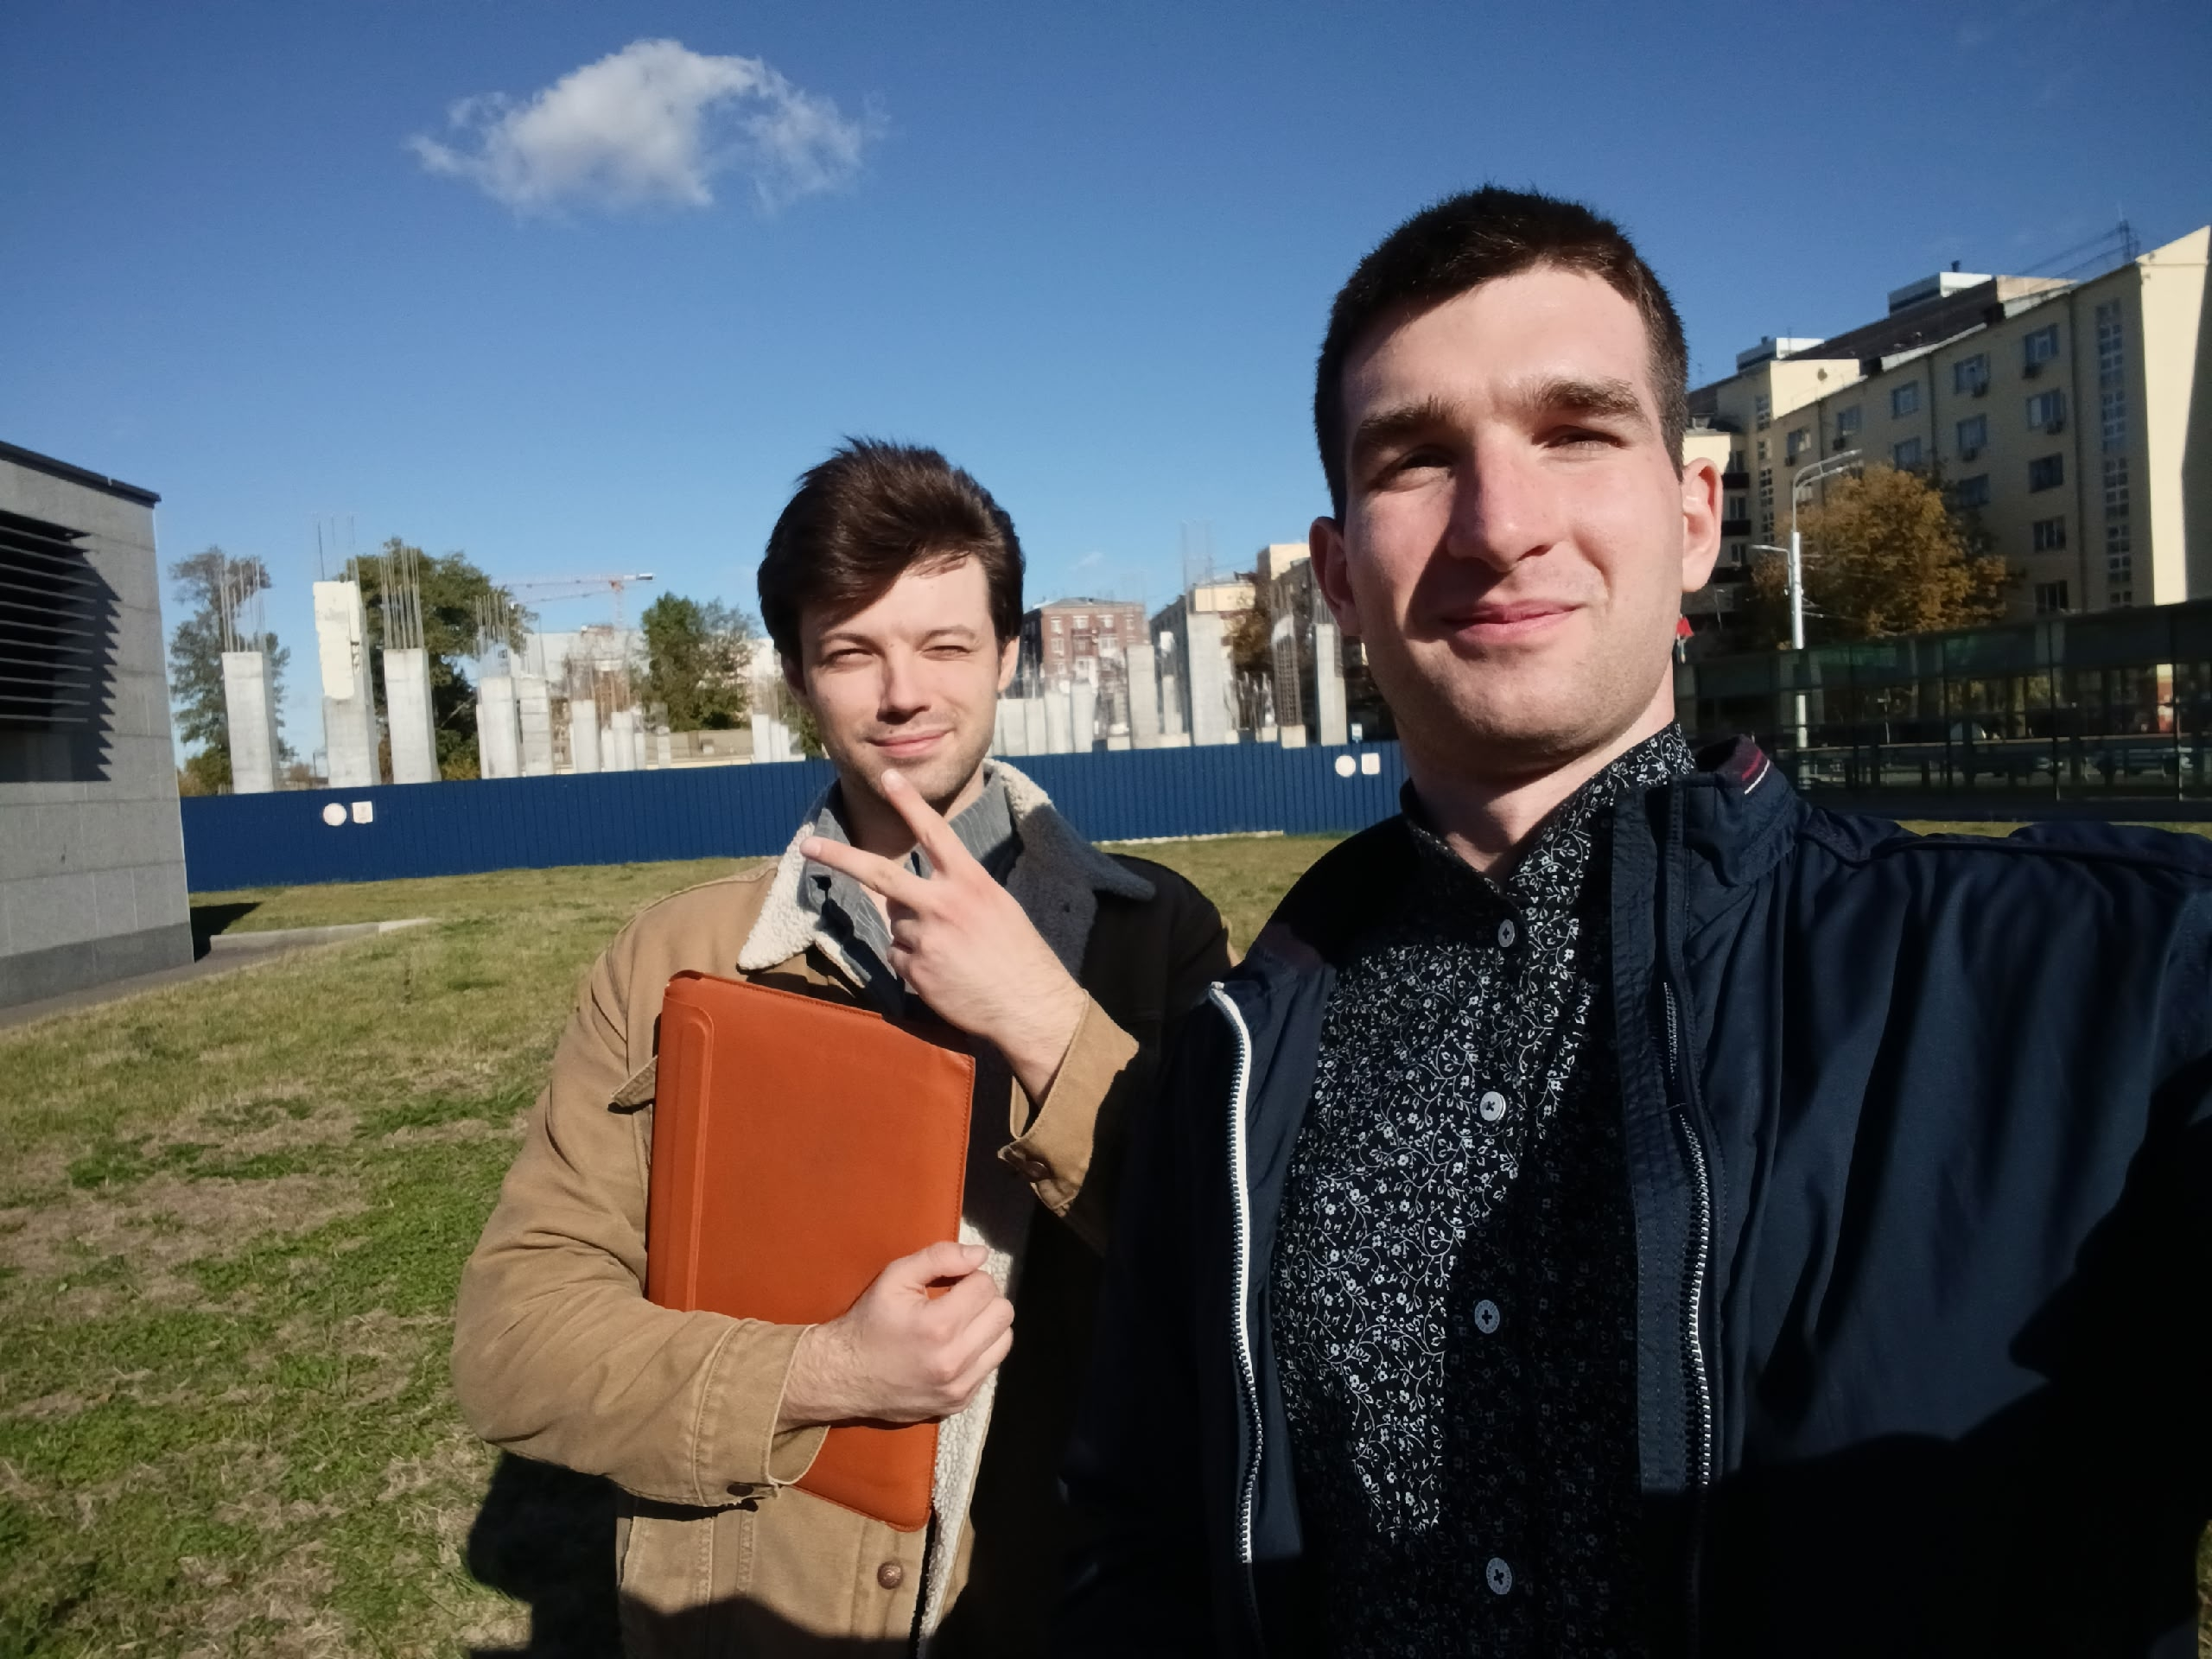
\includegraphics[height=6.2cm, keepaspectratio]{fig/selfie1_open.PNG}
        \caption{Фотофиксация на контрольной точке}
        \label{fig:selfie_open}
    \end{minipage}
    \hfill
    \begin{minipage}[b]{0.48\textwidth}
        \centering
        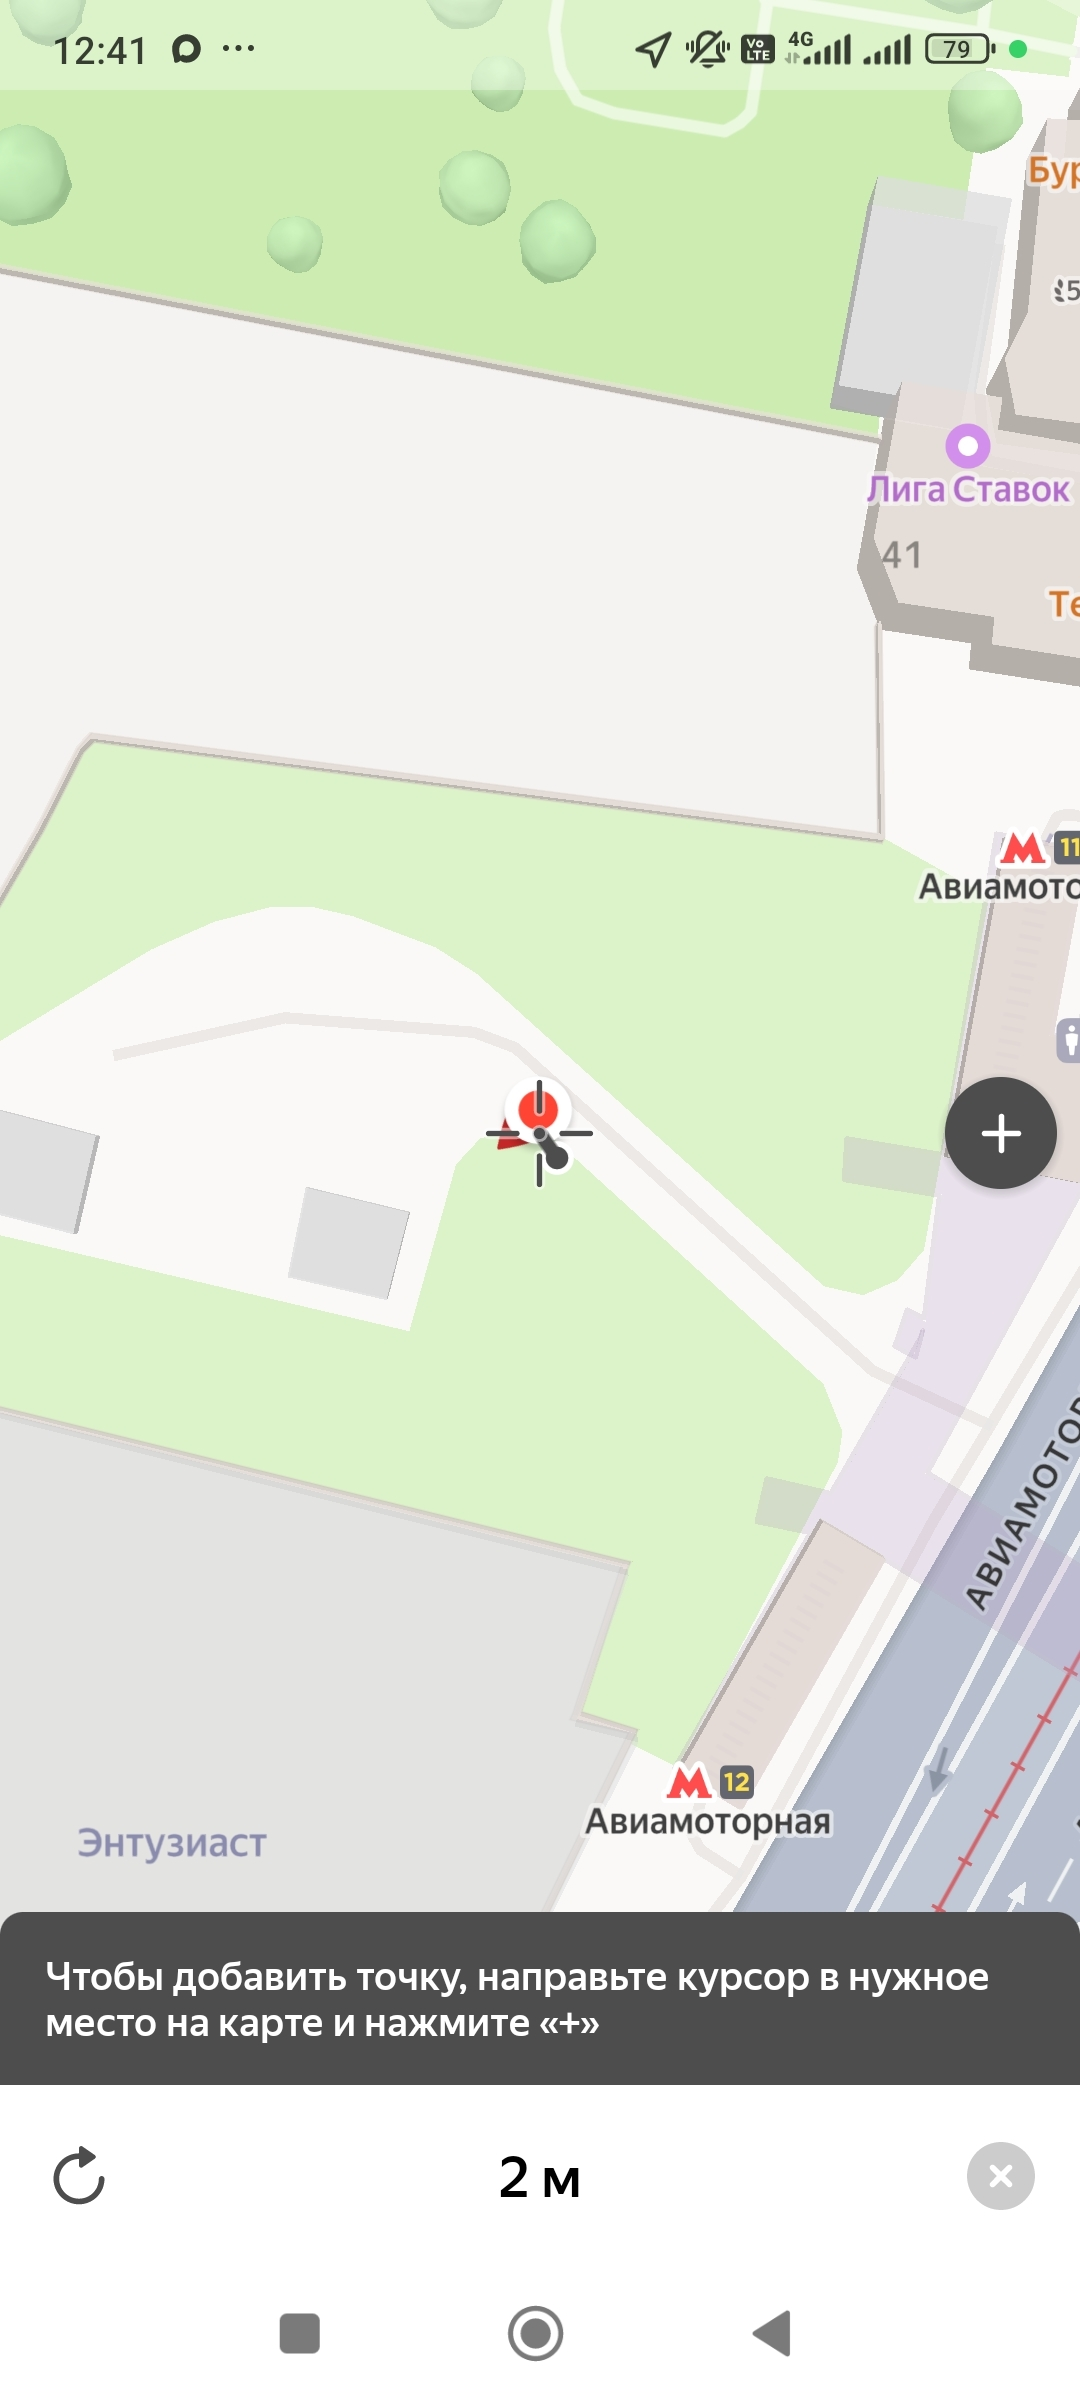
\includegraphics[height=6.2cm, keepaspectratio]{fig/maps1_open.PNG}
        \caption{Измерение погрешности на Яндекс Картах ($\Delta r = 2\text{ м}$)}
        \label{fig:map_open}
    \end{minipage}
\end{figure}

Полученная величина ошибки полностью укладывается в теоретическую точность базового режима абсолютных кодовых определений (SPP) для гражданской НАП. Высокая точность обусловлена минимальным влиянием переотраженных сигналов (многолучевости) и хорошим геометрическим фактором расположения видимых спутников на открытом горизонте.

\subsection{Оценка точности позиционирования в условиях малоэтажной застройки}

Вторая серия измерений проводилась вблизи малоэтажного здания. Присутствие искусственных преград частично ограничило сектор прямого обзора небосвода и создало условия для затенения низколетящих навигационных аппаратов.

В точке измерений были зафиксированы показания приемника смартфона и сделана контрольная фотография объекта. При последующем сравнении с фактическим ориентиром на геоинформационном сервисе «Яндекс Карты» линейное отклонение составило $7\text{ м}$, что заметно превышает погрешность на открытой площадке.

\begin{figure}[h!]
    \centering
    \begin{minipage}[b]{0.47\textwidth}
        \centering
        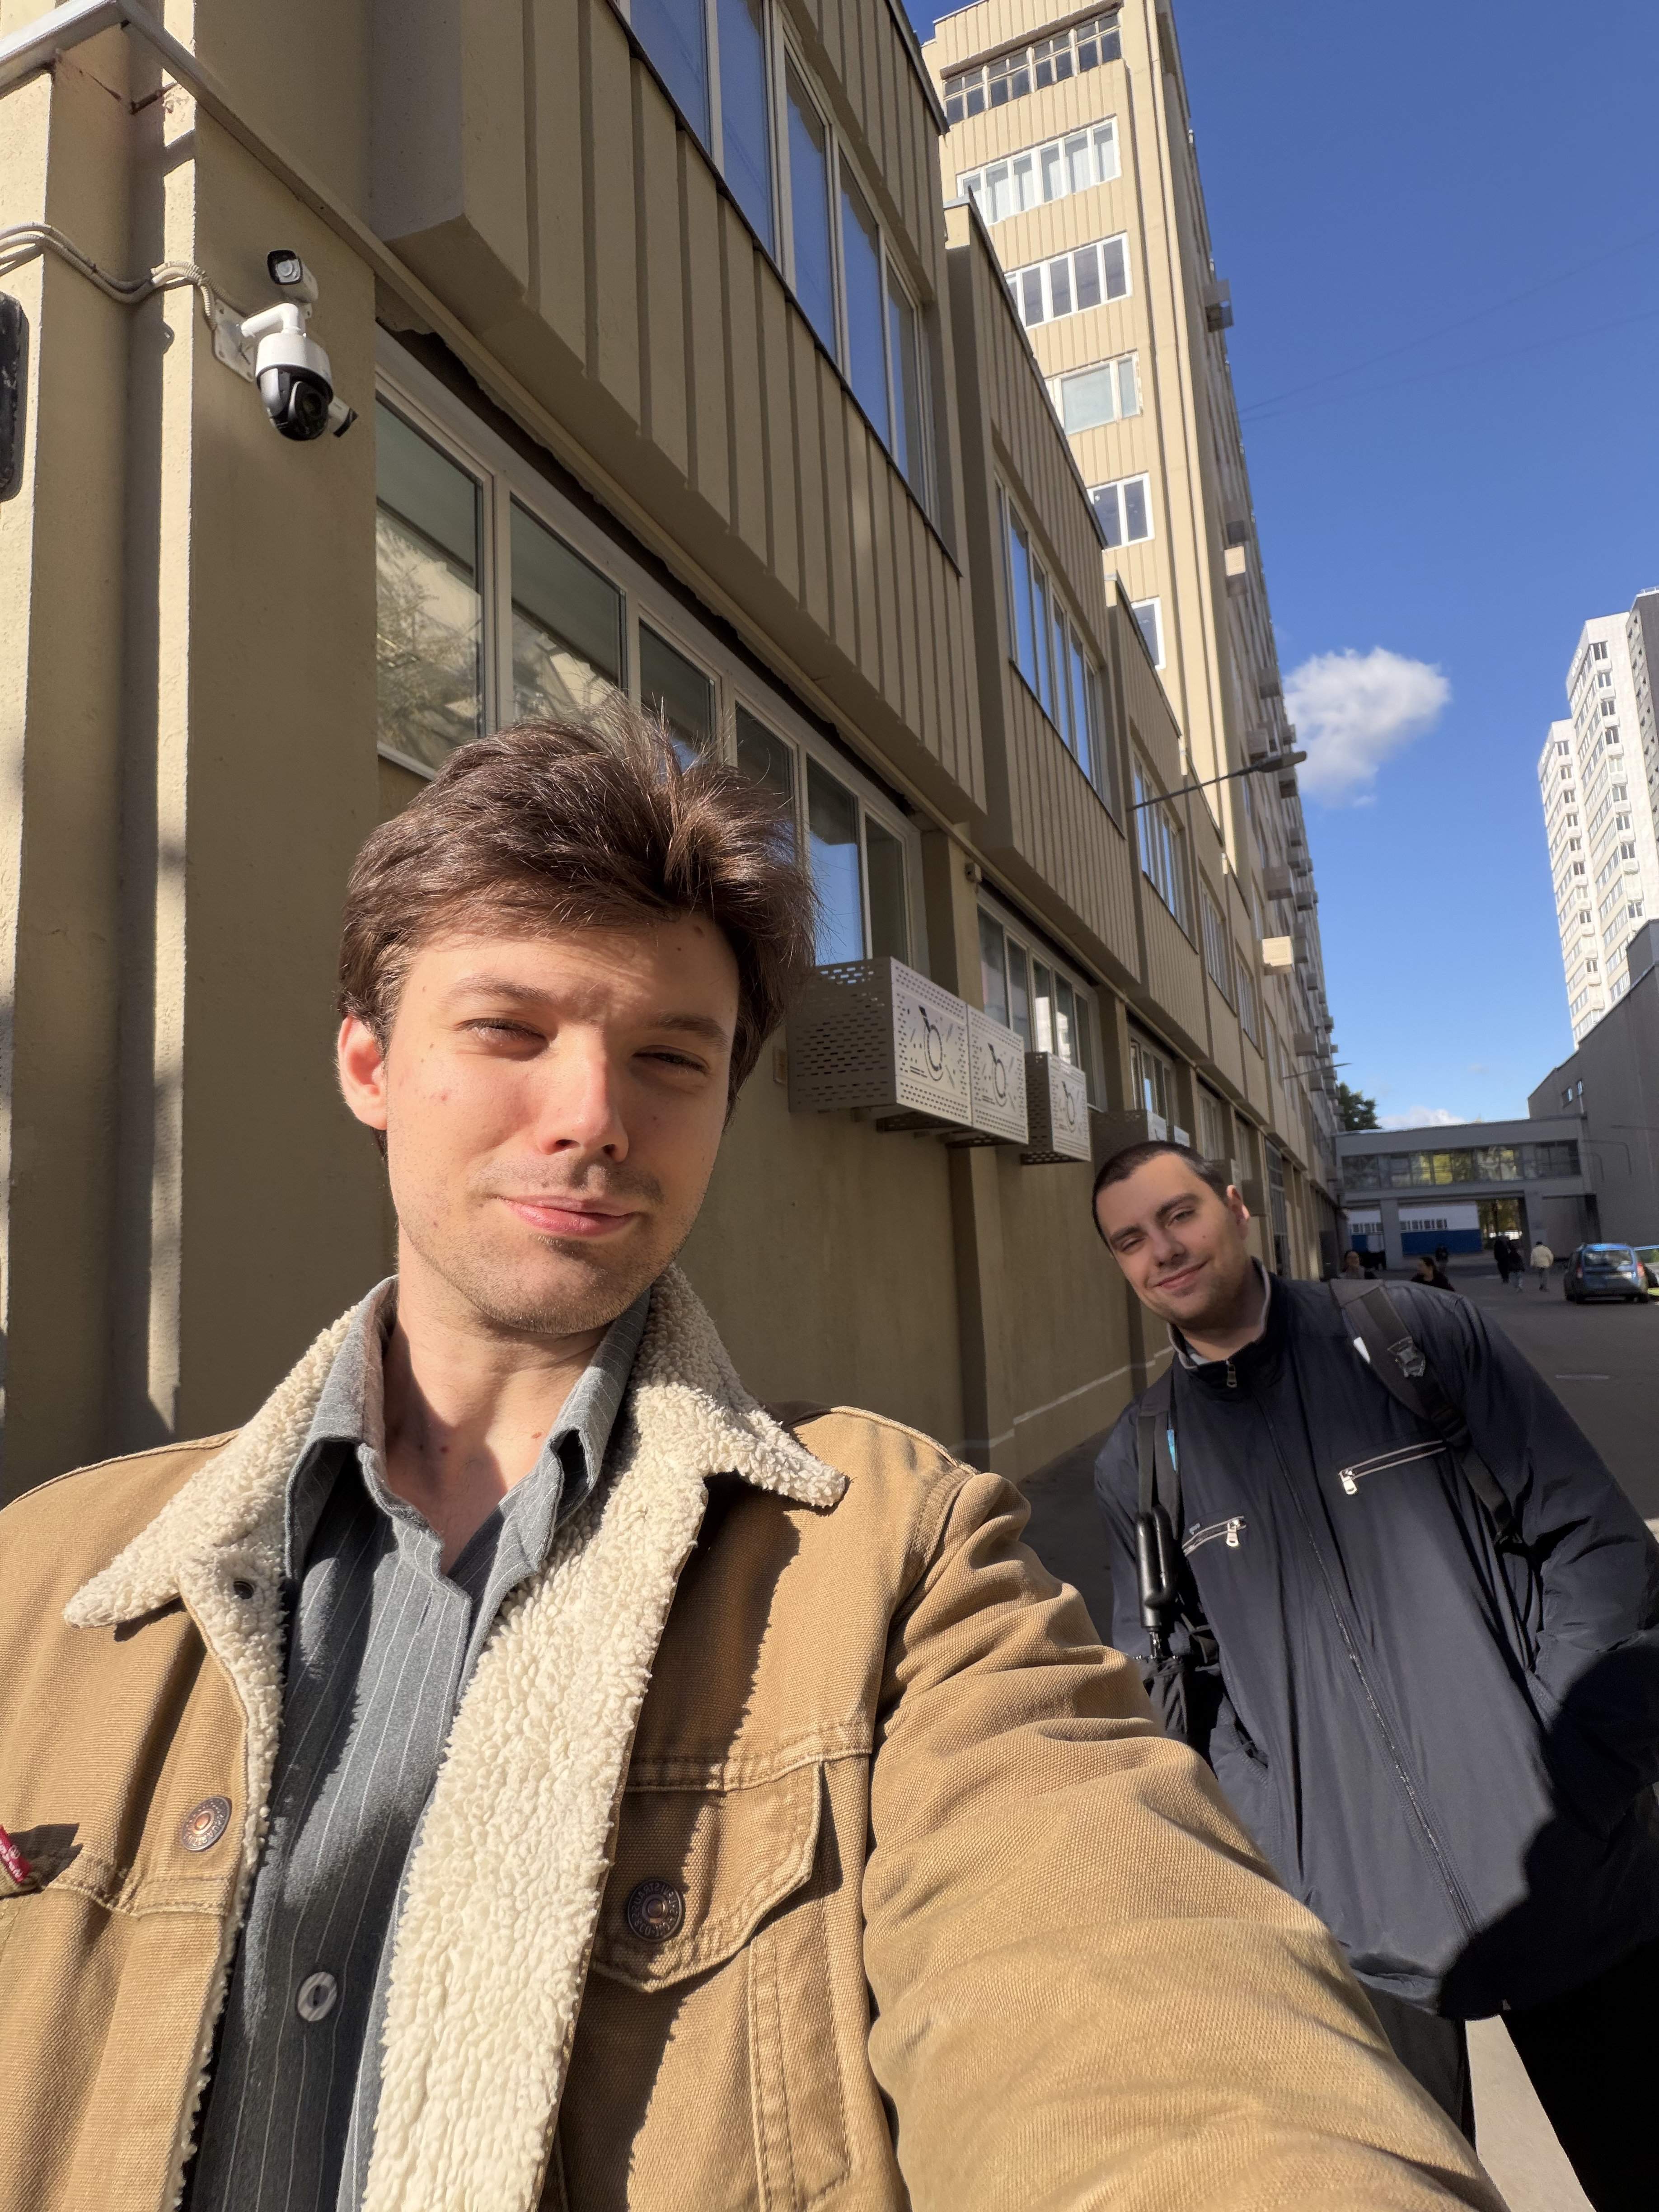
\includegraphics[width=\linewidth, keepaspectratio]{fig/selfie2_open.jpg}
        \caption{Фотофиксация вблизи малоэтажного здания}
        \label{fig:selfie_lowrise}
    \end{minipage}
    \hfill
    \begin{minipage}[b]{0.47\textwidth}
        \centering
        % Параметр trim срезает пустоту: left bottom right top
        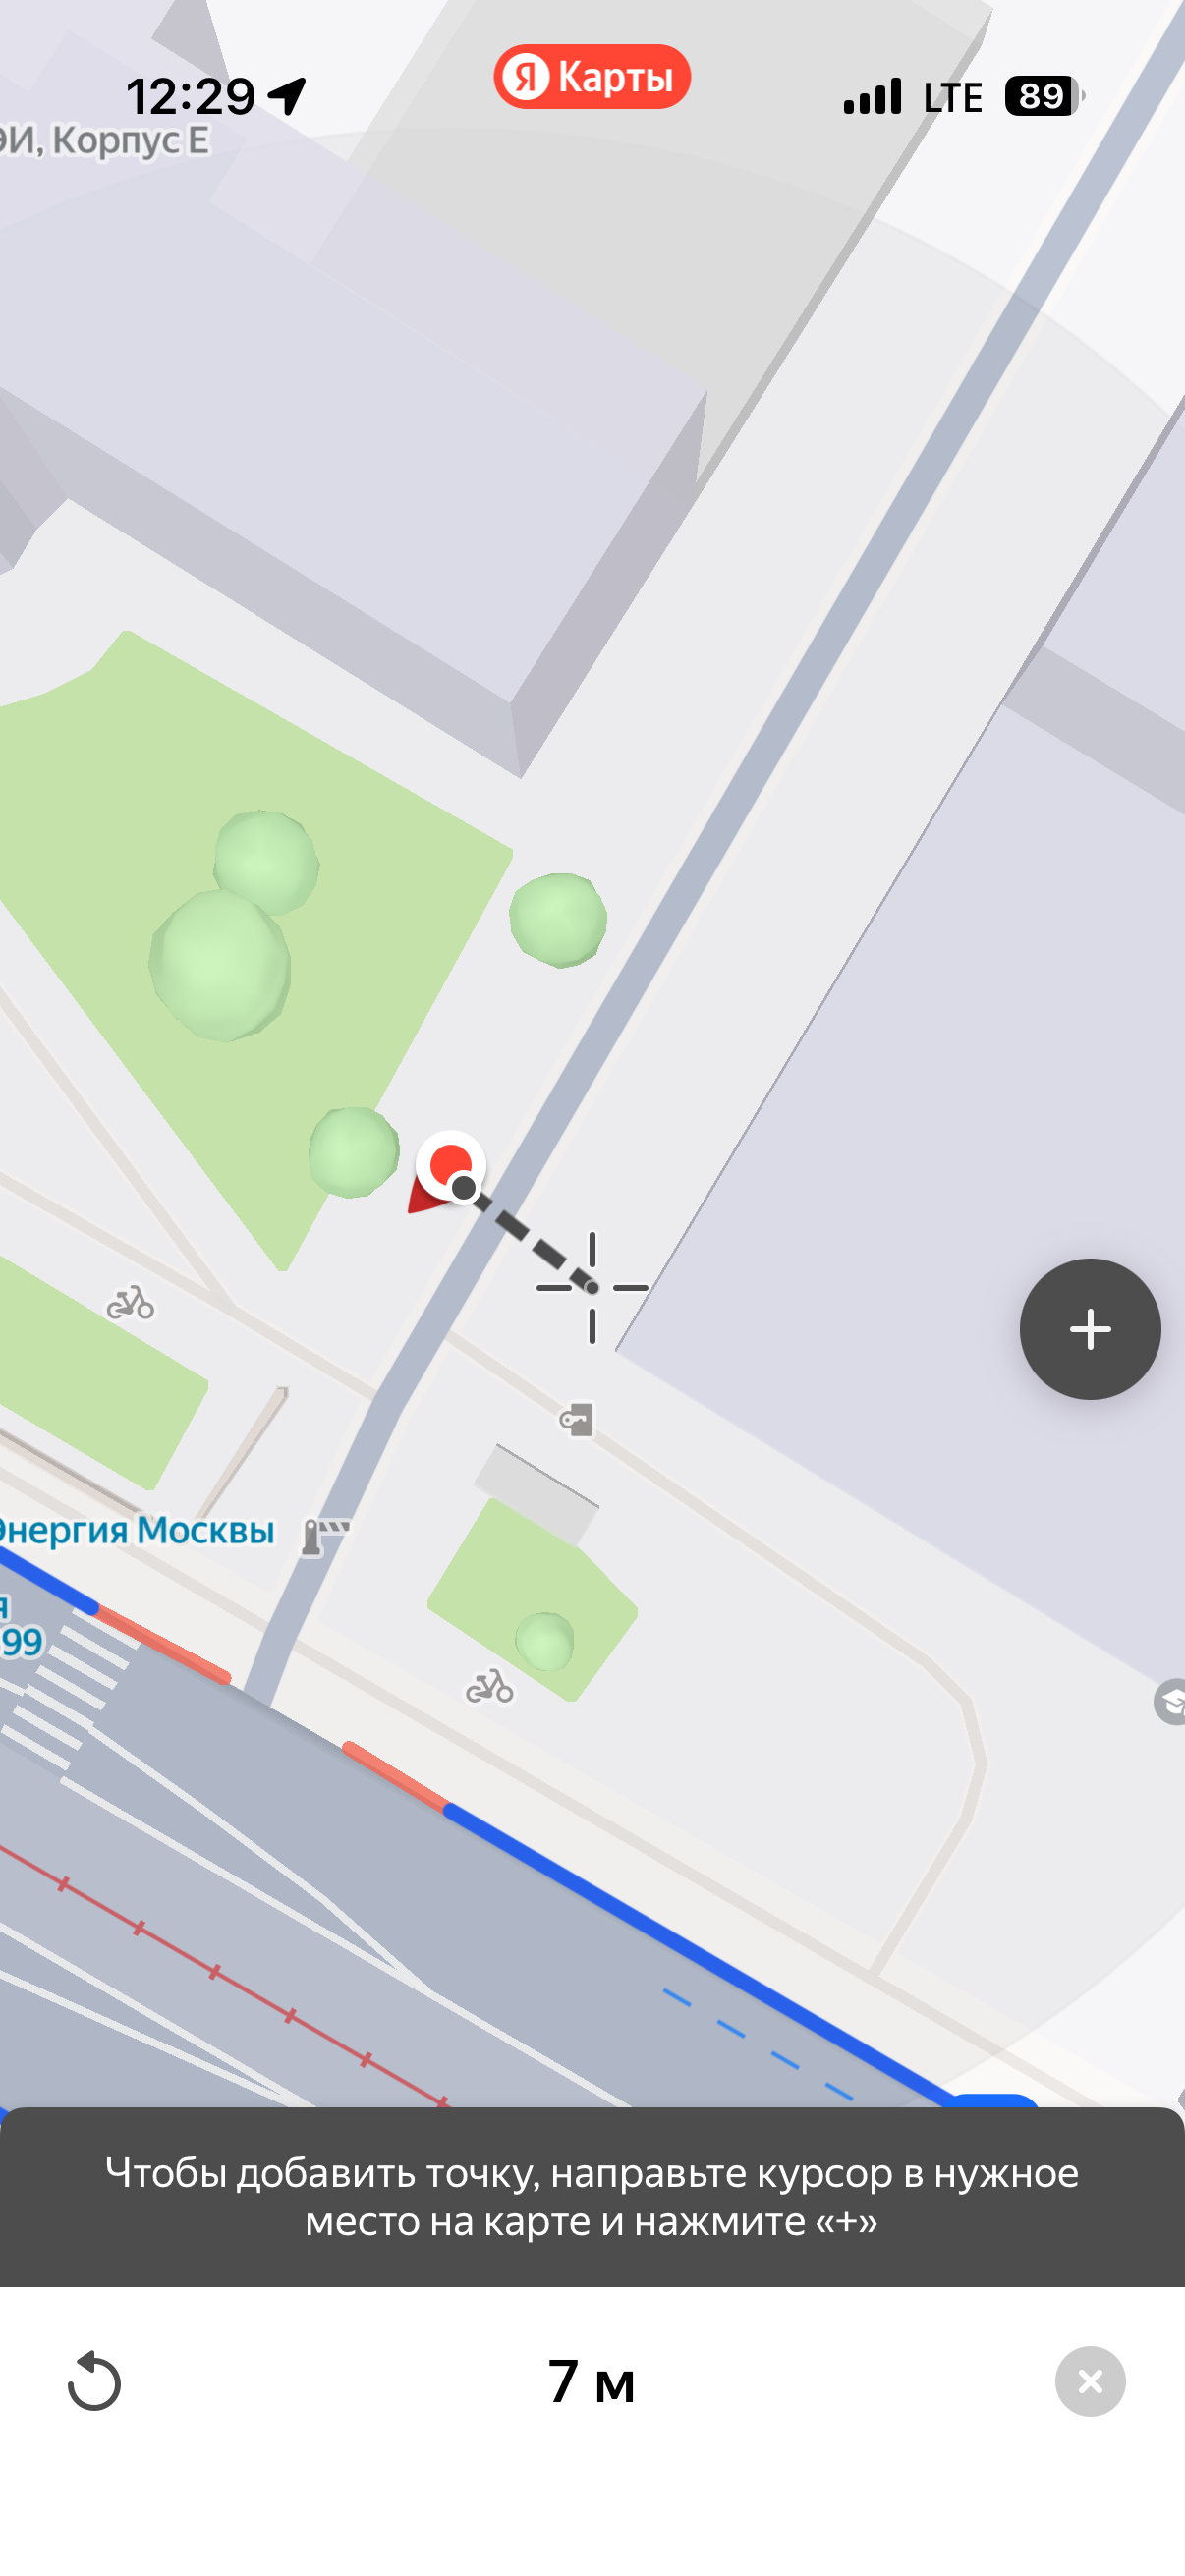
\includegraphics[width=0.82\linewidth, trim={0 3.5cm 0 2.5cm}, clip, keepaspectratio]{fig/maps2_open.PNG}
        \caption{Измерение погрешности на Яндекс Картах ($\Delta r = 7\text{ м}$)}
        \label{fig:map_lowrise}
    \end{minipage}
\end{figure}

Ухудшение точности обусловлено проявлением эффекта многолучевого распространения радиоволн из-за переотражений от стен постройки, а также ухудшением геометрического фактора расположения видимого созвездия спутников вследствие экранирования горизонта.

\subsection{Оценка точности позиционирования в условиях плотной высотной застройки}

Заключительная серия измерений проводилась в непосредственной близости от 9-этажного жилого здания. Условия приема радиосигналов характеризовались выраженным эффектом «городского каньона»: массивная вертикальная конструкция строения перекрыла значительную часть верхней полусферы, вызвав затенение большинства спутников рабочего созвездия с одной из сторон горизонта.

В контрольной точке были зафиксированы координаты приемника смартфона и выполнена привязка к ориентиру на местности. При сопоставлении с эталонным положением на сервисе «Яндекс Карты» линейное отклонение достигло максимального значения за весь эксперимент и составило $37\text{ м}$.

\begin{figure}[h!]
    \centering
    \begin{minipage}[b]{0.47\textwidth}
        \centering
        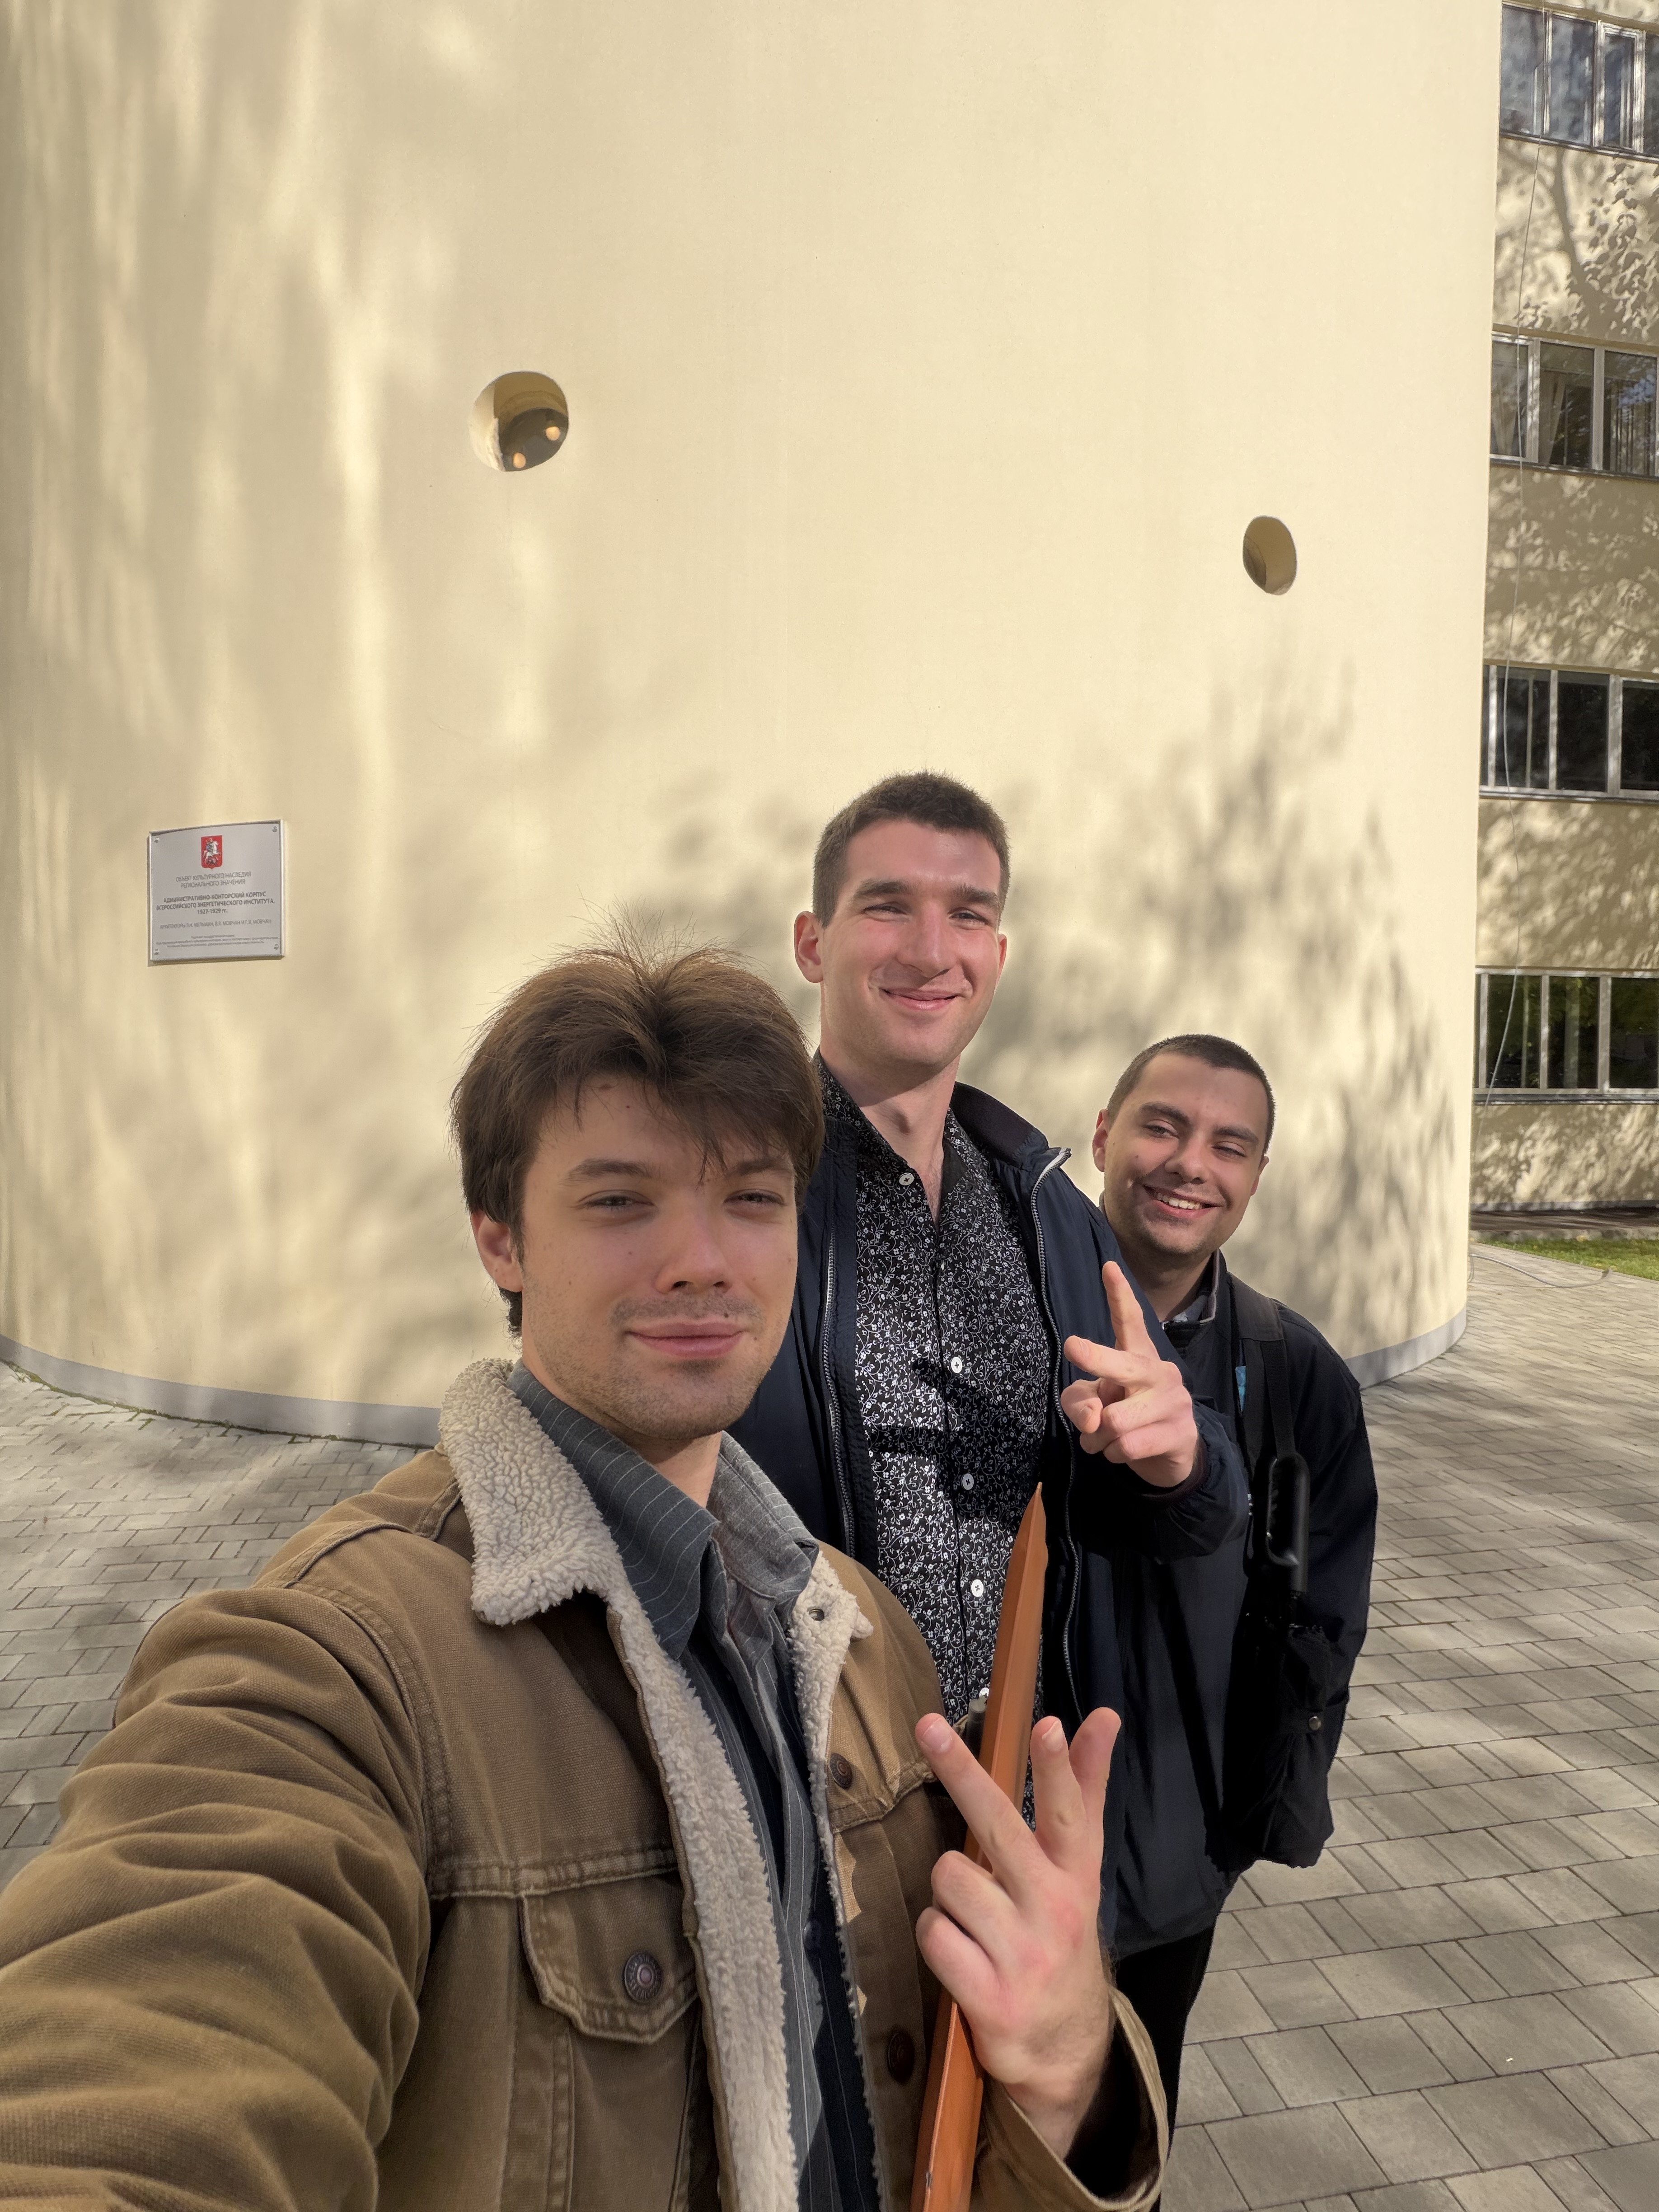
\includegraphics[width=\linewidth, keepaspectratio]{fig/selfie3_open.jpg}
        \caption{Фотофиксация вблизи 9-этажного здания}
        \label{fig:selfie_highrise}
    \end{minipage}
    \hfill
    \begin{minipage}[b]{0.47\textwidth}
        \centering
        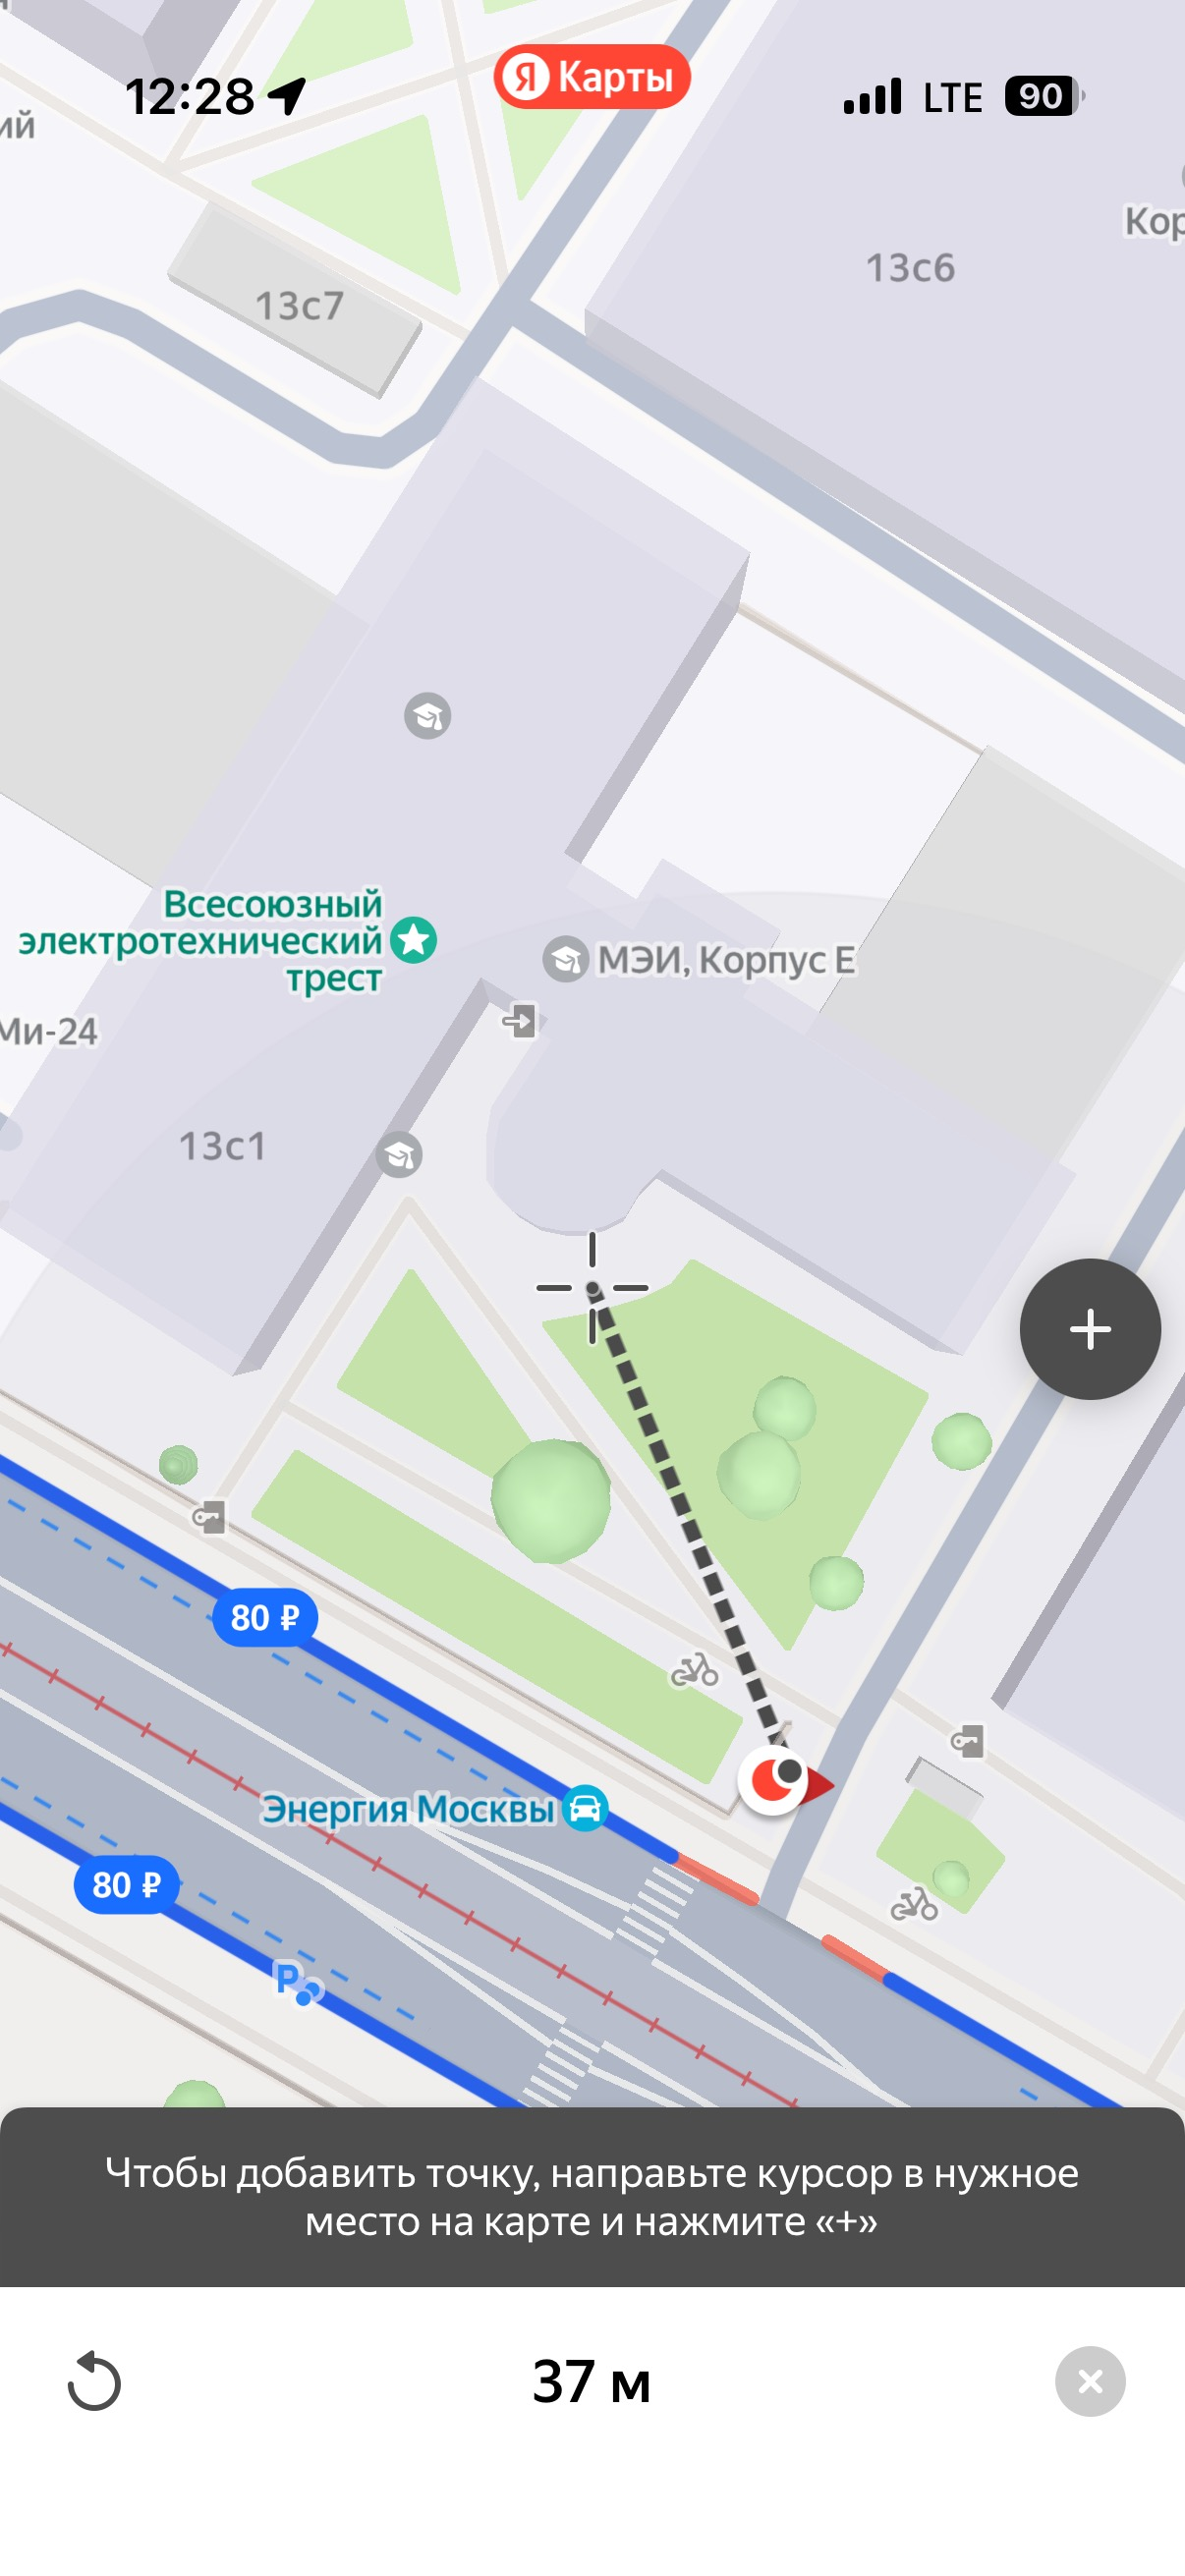
\includegraphics[width=0.82\linewidth, trim={0 3.5cm 0 2.5cm}, clip, keepaspectratio]{fig/maps3_open.jpg}
        \caption{Измерение погрешности на Яндекс Картах ($\Delta r = 37\text{ м}$)}
        \label{fig:map_highrise}
    \end{minipage}
\end{figure}

Столь существенная деградация точности обусловлена двумя ключевыми физическими факторами:
\begin{enumerate}
    \item \textbf{Интенсивная многолучевость:} сигналы от спутников, находящихся вне зоны прямой видимости, принимались после многократных переотражений от железобетонного фасада здания, что внесло аномальную задержку в псевдодальномерные измерения.
    \item \textbf{Ухудшение геометрии рабочего созвездия (рост GDOP/PDOP):} экранирование полусферы привело к тому, что навигационное решение строилось по ограниченной группе спутников, расположенных в узком телесном угле, что кратно усилило дисперсию погрешности позиционирования.
\end{enumerate}
